\section{Synthetic smoke test}
\label{app:smoke}

The Zipf topic mixtures have 20{,}000 documents in 64 dimensions. Four settings vary the number of topics (50, 200 or 500), the Zipf exponent and the noise. Each setting was run at three seeds and eleven sample sizes from 50 to 5{,}000. Table~\ref{tab:smoke} compares coverage $1 - G$ with the true topic mass coverage at radius $\alpha$ times the median pairwise distance of a pilot.

\begin{table}[h]
\centering
\small
\begin{tabular}{rrr}
\toprule
$\alpha$ & Spearman $\rho$ & mean absolute error \\
\midrule
0.5 & 0.968 & 0.029 \\
0.4 & 0.797 & 0.091 \\
0.3 & 0.677 & 0.209 \\
0.2 & 0.576 & 0.521 \\
0.1 & 0.307 & 0.869 \\
\bottomrule
\end{tabular}
\caption{Agreement of $1 - G$ with true topic coverage on the Zipf mixtures, 132 samples.}
\label{tab:smoke}
\end{table}

\section{The sample size formula by corpus}
\label{app:nstar}

Equation~\ref{eq:collapse} was fitted on cells with $n \le 1{,}000$, five draws per cell. Equation~\ref{eq:nstar} then gave $n^{*}$ for $\varepsilon \in \{0.3, 0.2, 0.1\}$ at every radius where the mean surface crosses $\varepsilon$ at some $n > 1{,}000$, and the crossing was interpolated on the log scale between grid points. Table~\ref{tab:nstar} reports the ratio of predicted to empirical sample size. The grid steps by a factor of about 1.5 between adjacent sample sizes, and the interpolated crossing varies across the five draws by a median of 6\%. Leaving out the Zipf mixture, 10 of the 18 cases on failing text pairs fall within a factor of 1.5 and 14 within 2. With $a$ and $b$ fitted on nested subsamples of one 2{,}000-document pilot instead of draws from the whole corpus, 76 of the 83 cases on passing pairs fall within 1.5 and 81 within 2.

\begin{table}[h]
\centering
\small
\begin{tabular}{llrrrr}
\toprule
Corpus & Enc. & cases & median & $\le 1.5$ & $\le 2$ \\
\midrule
AskDocs & Qwen3 & 5 & 1.04 & 5 & 5 \\
Truth Social & Qwen3 & 6 & 0.88 & 5 & 6 \\
Census random & Qwen3 & 3 & 0.81 & 2 & 2 \\
Manifold $d{=}2$ & none & 9 & 1.15 & 9 & 9 \\
TIFU & Qwen3 & 6 & 1.08 & 6 & 6 \\
Bluesky & Qwen3 & 5 & 0.74 & 3 & 4 \\
TIFU & GTR & 17 & 1.24 & 17 & 17 \\
Manifold $d{=}8$ & none & 7 & 1.12 & 7 & 7 \\
AskDocs & GTR & 16 & 0.96 & 14 & 16 \\
Manifold $d{=}4$ & none & 9 & 1.09 & 9 & 9 \\
\midrule
Census illegal & Qwen3 & 3 & 1.24 & 2 & 3 \\
Census covid & Qwen3 & 3 & 1.22 & 3 & 3 \\
Trump & Qwen3 & 2 & 1.14 & 2 & 2 \\
Census trump & Qwen3 & 2 & 1.56 & 1 & 2 \\
Census citizens & Qwen3 & 2 & 2.06 & 0 & 1 \\
Trump & GTR & 6 & 1.86 & 2 & 3 \\
Zipf, 200 topics & none & 5 & 69 & 0 & 0 \\
\bottomrule
\end{tabular}
\caption{Predicted over empirical sample size for a target isolation rate, in the order of Table~\ref{tab:collapse}. GTR rows pool three samples of the forum corpus.}
\label{tab:nstar}
\end{table}

\section{Coverage of a theme inventory}
\label{app:themes}

Each of the eight forum and census corpora received inventories of themes by $k$-means on the full Qwen3 embeddings at $K = 10$, 30 and 100, and two inventories with skewed masses at $K = 30$: one from $k$-means++ seeding without refinement, one by merging the 100 clusters into 30 groups of Zipf sizes. The effective number of themes (the exponential of the entropy of the masses) ranges from 6.8 to 91. For each inventory and the 1{,}200 samples of Section~\ref{app:summaries}, Table~\ref{tab:themes} gives the range across corpora of the share of theme mass present. The expected coverage $\sum_k m_k (1 - (1 - m_k)^{n})$ matches the observed value to a mean absolute error of 0.004 over all cells. For the $K = 30$ inventory, Gemma~4 \citep{gemma4} was shown each sample and the list of named themes and asked which were present, with a supporting document for each. The mass of themes it reported rose with $n$ along the label coverage curve in every corpus, and the share of its reports that the labels confirm rose from 0.73 at $n = 25$ to 0.98 at $n = 400$.

\begin{table}[h]
\centering
\small
\begin{tabular}{lccc}
\toprule
Inventory & $n{=}25$ & $n{=}50$ & $n{=}100$ \\
\midrule
$k$-means, $K{=}10$ & 0.89 to 0.94 & 0.98 to 1.00 & 1.00 \\
$k$-means, $K{=}30$ & 0.58 to 0.64 & 0.82 to 0.85 & 0.94 to 0.98 \\
$k$-means, $K{=}100$ & 0.25 to 0.30 & 0.44 to 0.48 & 0.67 to 0.72 \\
seeding only, $K{=}30$ & 0.60 to 0.72 & 0.82 to 0.88 & 0.94 to 0.96 \\
Zipf merge, $K{=}30$ & 0.79 to 0.84 & 0.87 to 0.91 & 0.93 to 0.96 \\
\bottomrule
\end{tabular}
\caption{Share of theme mass present in a sample, range across eight corpora.}
\label{tab:themes}
\end{table}

\begin{figure}[h]
\centering
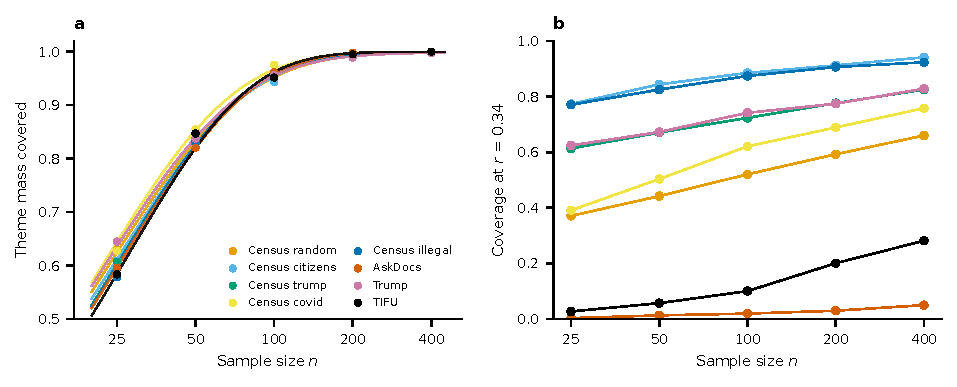
\includegraphics[width=\columnwidth]{figures/themes.pdf}
\caption{(a) Share of theme mass present in a sample against $n$ for the $K = 30$ inventory, eight corpora (points), with the expected coverage from each corpus's masses (lines). (b) Coverage $1 - G$ at the fixed radius $r = 0.34$ for the same samples.}
\label{fig:themes}
\end{figure}

\section{Summary stability}
\label{app:summaries}

For each of the eight forum and census corpora and each $n \in \{25, 50, 100, 200, 400\}$, thirty independent samples were summarized by Gemma~4 at temperature 0 in one paragraph of at most 150 words, and the summaries were embedded with Qwen3-Embedding-8B. Instability is the mean pairwise cosine distance among the thirty summaries. Within every corpus instability falls with $n$ and tracks $G$ (Spearman $+0.40$ to $+1.00$, seven of eight at $+0.70$ or above). Across corpora at a fixed $n$, Spearman of instability with $G$ is $+0.14$, $+0.12$, $+0.12$, $+0.07$ and $-0.17$ at $n = 25$ to 400, with bootstrap bands that include zero. TIFU illustrates why: its $G$ is near 1 at the shared radius and its summaries are the most stable, because the model summarizes it as stories of mishap whichever thirty stories it is given.

\section{A bound for functions that are stable at scale $r$}
\label{app:bound}

For a document function $f$ with range 1 that takes the same value on documents within $r$ of each other, the estimate of the corpus mean of $f$ formed by giving each corpus document the value of its nearest sampled document errs by at most $v(r) + M(r)$, where $v(r)$ is the share of covered documents whose nearest sampled document disagrees with them on $f$. On fifty cluster indicator functions over four corpora, six sample sizes and six radii, the bound held in 144 of 144 cells and was loose for proportions (median 22 times the realised error), where the plain sample mean already errs by 0.003 to 0.07.

\section{Prompts}
\label{app:prompts}

\paragraph{Summary.} ``Below are $\{n\}$ documents sampled from a larger collection. Write a summary of the collection in one paragraph of at most 150 words. Cover the main themes in proportion to how often they appear, name notable minority themes briefly, and do not mention individual document numbers.''

\paragraph{Theme naming.} ``The $\{m\}$ documents below were grouped together because they are about the same theme. Give the theme a short name (at most 8 words) and a one-sentence definition that would let a reader decide whether a new document belongs to it. Answer as JSON with keys name and definition.''

\paragraph{Enumeration.} ``Below are $\{n\}$ documents sampled from a larger collection, followed by a list of $\{K\}$ themes found in the full collection. Decide which themes are present among these $\{n\}$ documents. A theme is present only if you can point to one document that is primarily about it; in a small sample most themes will be absent, and similar-sounding themes are distinct, so pick the single best theme for each document. Answer with one line per present theme in the form theme\_id: document\_number.''

\paragraph{Same content.} ``Two documents from the same collection are shown. Judge their relation. SAME: they are about the same specific content (the same claim, question, event or story), so a reader who has read one would learn little new from the other. TOPIC: they are about the same general topic but different specific content. UNRELATED: they are about different topics.''
